\documentclass[border=8pt]{standalone}
\usepackage{xcolor}
\definecolor{deepblue}{RGB}{31,84,150}
\definecolor{steel}{RGB}{70,130,180}
\definecolor{crimsonred}{RGB}{190,30,60}
\definecolor{darkorang}{RGB}{230,140,20}
\usepackage{pgfplots}
\pgfplotsset{compat=1.18}
\begin{document}
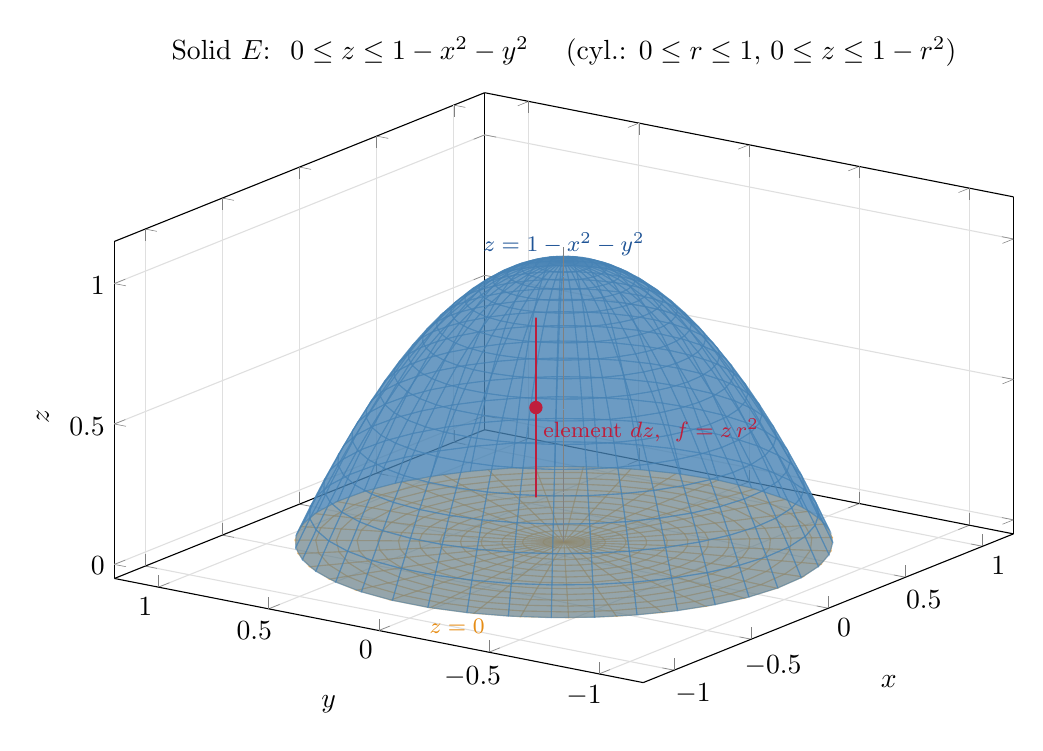
\begin{tikzpicture}
\begin{axis}[
    view={-55}{22},
    width=13cm, height=10.5cm,
    xmin=-1.2, xmax=1.2, ymin=-1.2, ymax=1.2, zmin=-0.05, zmax=1.15,
    xlabel={$x$}, ylabel={$y$}, zlabel={$z$},
    z post scale=0.75,
    grid=major, grid style={gray!25},
    title={Solid $E$: $\;0\le z\le 1-x^2-y^2$ \quad (cyl.: $0\le r\le1$, $0\le z\le1-r^2$)},
    every title/.append style={font=\small},
]
% --- base disk  z = 0 -------------------------------------------------------
\addplot3[surf, color=darkorang, opacity=0.40, shader=flat,
          samples=14, samples y=36, domain=0:1, y domain=0:360]
    ({x*cos(y)}, {x*sin(y)}, {0});
% --- paraboloid cap  z = 1 - r^2 -------------------------------------------
\addplot3[surf, color=steel, opacity=0.55, shader=flat,
          samples=20, samples y=40, domain=0:1, y domain=0:360]
    ({x*cos(y)}, {x*sin(y)}, {1-x^2});
% --- z-axis -----------------------------------------------------------------
\addplot3[gray, dashed, thin, domain=0:1.05, samples=2] ({0},{0},{x});
% --- representative vertical element dz at r = 0.6, theta = 45deg -----------
\addplot3[thick, crimsonred, domain=0:0.64, samples=2]
    ({0.6*cos(45)},{0.6*sin(45)},{x});
\addplot3[only marks, mark=*, mark size=2.2, color=crimsonred]
    coordinates {(0.4243,0.4243,0.32)};
\node[crimsonred, font=\footnotesize, anchor=north west] at (axis cs:0.46,0.46,0.30)
    {element $dz$,\; $f=z\,r^2$};
% --- labels on the two bounding surfaces ------------------------------------
\node[deepblue, font=\footnotesize] at (axis cs:0,0,1.06) {$z=1-x^2-y^2$};
\node[darkorang, font=\footnotesize] at (axis cs:-1.05,-0.25,-0.03) {$z=0$};
\end{axis}
\end{tikzpicture}
\end{document}
